\documentclass[12pt,onecolumn,a4paper]{article}
\usepackage{epsfig,graphicx,subcaption,amsthm,amsmath}
\usepackage{float}
\usepackage{color,xcolor}
\usepackage{fmtcount}
\usepackage{placeins}
\usepackage{adjustbox}
\usepackage{tikz}
\usepackage{csvsimple}
\usepackage[top=1in, left=1in, right=1in, bottom=1in]{geometry}




%\usepackage{lmodern}
%\usepackage[T1]{fontenc}
%\usepackage[utf8]{i.nputenc}


%\definecolor{seccolor}{RGB}{41,48,57}
%\titleformat{\section}
%[hang]
%{\Large\bfseries}
%{}
%{0pt}
%{\tikz{
		%		\node[draw, rounded corners=1mm,text depth=0.2ex,line width=2pt,anchor=west](a){\Large\bfseries\textcolor{seccolor}{}#1};
		%		\coordinate (b) at (\textwidth-2em,0);
		%		\draw[line width=2pt] (a)--(b);}}


%\titleformat{\section}
%{\titlerule     
	%	\vspace{0.5ex}%
	%	\sectionfont}
%{\bfseries\thesection}{1em}
%{\sectionfont}[\titlerule]

%\usepackage[utf8]{inputenc}
\usepackage{titlesec}
\titleformat{\section}[block]
{\titlerule\addvspace{4pt}\normalfont\fontsize{14}{16}\bfseries}
{\thesection\enspace}{0pt}{}[\vspace{2pt}\titlerule]


%\usepackage{xepersian}
%\settextfont[Scale=1.2]{B Nazanin}
%\setlatintextfont[Scale=1]{Times New Roman}
%\setmathdigitfont{Yas}

%\newcommand\question{\section{سوال \tartibi{section}}}
\newcommand\question{
	%	\noindent\rule{\linewidth}{1}
	\section{Question \numberstringnum{\thesection}:}
	%	\rule{\linewidth}{1}
}


\author{Mohammad Raziei}
\title{Solutions to the First Series of Exercises}
\date{\today}

\begin{document}
	\maketitle
	
	
	%%%%%%%%%%%%%%%%%%%%%%%%%%%%%%%%%%%%%%%%%%%%%%%%%%%%%%%%%%%%%%%%%%%%
	\FloatBarrier\question%1
	%%%%%%%%%%%%%%%%%%%%%%%%%%%%%%%%%%%%%%%%%%%%%%%%%%%%%%%%%%%%%%%%%%%%
	
	
	
	\begin{figure}[h]
		
		\begin{subfigure}{\linewidth}
			\centering
			\begin{adjustbox}{scale=1.2}
				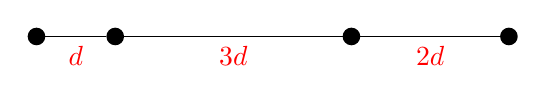
\begin{tikzpicture}[scale=1, every node/.style={scale=1}]
					\def\dscale{1}
					\foreach \vertexold/\vertex in {0/0, 0/1, 1/4, 4/6} {
						\node[draw,circle,fill=black, inner sep=2pt,line width=.7] (\vertex) at (\dscale*\vertex, 0) {};
						
						% Draw a line and add the difference label if vertexold is less than vertex
						\ifnum\vertexold<\vertex
						\pgfmathsetmacro\difference{\vertex - \vertexold} % Calculate the difference
						
						% Format the output based on whether it is an integer or not
						% Format the output based on whether it is an integer or not
						\pgfmathsetmacro\differenceDisplay{int(\difference) == \difference ? int(\difference) : \difference}
						
						% Decide on what to display
						\pgfmathsetmacro\displayText{\differenceDisplay == 1 ? "" : \differenceDisplay}
						
						
						% Draw the line and display the difference
						\draw (\vertexold) -- (\vertex) node[midway, below, red] {$\displayText d$};
						\fi
					}
				\end{tikzpicture}
			\end{adjustbox}
			\caption{}
		\end{subfigure}
		
		\vspace{1.5em}
		
		\begin{subfigure}{\linewidth}
			\centering
			\begin{adjustbox}{scale=1.2}
				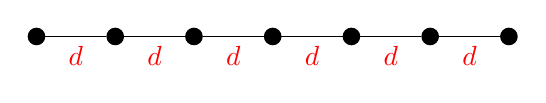
\begin{tikzpicture}[scale=1, every node/.style={scale=1}]
					\def\dscale{1}
					\foreach \vertexold/\vertex in {0/0, 0/1, 1/2, 2/3, 3/4, 4/5, 5/6} {
						\node[draw,circle,fill=black, inner sep=2pt,line width=.7] (\vertex) at (\dscale*\vertex, 0) {};
						
						% Draw a line and add the difference label if vertexold is less than vertex
						\ifnum\vertexold<\vertex
						\pgfmathsetmacro\difference{\vertex - \vertexold} % Calculate the difference
						
						% Format the output based on whether it is an integer or not
						% Format the output based on whether it is an integer or not
						\pgfmathsetmacro\differenceDisplay{int(\difference) == \difference ? int(\difference) : \difference}
						
						% Decide on what to display
						\pgfmathsetmacro\displayText{\differenceDisplay == 1 ? "" : \differenceDisplay}
						
						
						% Draw the line and display the difference
						\draw (\vertexold) -- (\vertex) node[midway, below, red] {$\displayText d$};
						\fi
					}
				\end{tikzpicture}
			\end{adjustbox}
			\caption{}
		\end{subfigure}
		\caption{}
	\end{figure}
	
	
	\begin{figure}[h]
		\begin{subfigure}{.48\linewidth}
			\centering
			\includegraphics[width=\linewidth]{Q1/results/AF-plot}
			\caption{}
			\label{fig:af-plot}
		\end{subfigure}
		\hfill
		\begin{subfigure}{.48\linewidth}
			\centering
			\includegraphics[width=\linewidth]{Q1/results/AF-plot-logy}
			\caption{}
			\label{fig:af-plot-logy}
		\end{subfigure}
		\caption{
			\space
		}
	\end{figure}
	
	
	\begin{figure}
		\centering
		\includegraphics[width=.6\linewidth]{Q1/results/AF-polarplot}
		\caption{}
		\label{fig:af-polarplot}
	\end{figure}
	
	
	
	\begin{figure}
		\centering
		\begin{subfigure}{\linewidth}
			\centering
			\includegraphics[width=\linewidth]{Q1/results/AF-plot-localmaxmin-a}
			\caption{}
			\label{fig:af-plot-localmaxmin-a}
		\end{subfigure}
		
		\begin{subfigure}{\linewidth}
			\centering
			\includegraphics[width=\linewidth]{Q1/results/AF-plot-localmaxmin-b}
			\caption{}
			\label{fig:af-plot-localmaxmin-b}
		\end{subfigure}
		
		\caption{
			\space
		}
	\end{figure}
	
	
	
	%%%%%%%%%%%%%%%%%%%%%%%%%%%%%%%%%%%%%%%%%%%%%%%%%%%%%%%%%%%%%%%%%%%%
	\FloatBarrier\question%2
	%%%%%%%%%%%%%%%%%%%%%%%%%%%%%%%%%%%%%%%%%%%%%%%%%%%%%%%%%%%%%%%%%%%%
	
	
	\FloatBarrier
	\subsection{part a:}
	
	
	\FloatBarrier
	\subsection{part b:}
	
	
	\begin{figure}[h]
		\begin{subfigure}{.43\linewidth}
			\centering
			\includegraphics[width=\linewidth]{Q2/results/2d-plot-angles}
			\caption{}
			\label{fig:2d-plot-angles}
		\end{subfigure}
		\hfill
		\begin{subfigure}{.5\linewidth}
			\centering
			\includegraphics[width=\linewidth]{Q2/results/3d-plot-angles}
			\caption{}
			\label{fig:3d-plot-angles}
		\end{subfigure}
	\end{figure}
	
	
	\begin{figure}[h]
		\centering
		\includegraphics[width=0.7\linewidth]{Q2/results/spatial-antenna-pattern}
		\caption{}
		\label{fig:spatial-antenna-pattern}
	\end{figure}
	
	\FloatBarrier
	\subsection{part c:}
	
	\begin{figure}[h]
		\centering
		\includegraphics[width=0.4\linewidth]{Q2/results/phi0-polar}
		\caption{}
		\label{fig:phi0-polar}
	\end{figure}
	
	
	\begin{figure}[h]
		\centering
		\includegraphics[width=\linewidth]{Q2/results/phi0}
		\caption{}
		\label{fig:phi0}
	\end{figure}
	
	\FloatBarrier
	\subsection{part d:}
	
	
	
	\begin{figure}[h]
		\centering
		\includegraphics[width=0.4\linewidth]{Q2/results/phi90-polar}
		\caption{}
		\label{fig:phi90-polar}
	\end{figure}
	
	
	\begin{figure}[h]
		\centering
		\includegraphics[width=\linewidth]{Q2/results/phi90}
		\caption{}
		\label{fig:phi90}
	\end{figure}
	
	
	
	\FloatBarrier
	\subsection{part e:}
	
	
	
	
	\FloatBarrier
	\subsection{part f:}
	
	
	%%%%%%%%%%%%%%%%%%%%%%%%%%%%%%%%%%%%%%%%%%%%%%%%%%%%%%%%%%%%%%%%%%%%
	\FloatBarrier
	\question%3
	%%%%%%%%%%%%%%%%%%%%%%%%%%%%%%%%%%%%%%%%%%%%%%%%%%%%%%%%%%%%%%%%%%%%
	
	
		
	\FloatBarrier
	\subsection{part a:}
	
	
		
	\FloatBarrier
	\subsection{part b:}
	
	\begin{figure}[h]
		\centering
		\begin{subfigure}{.45\linewidth}
			\centering
			\includegraphics[width=\linewidth]{Q3/results/s11}
			\caption{$S_{11}$}
			\label{fig:s11}
		\end{subfigure}
		\hfill
		\begin{subfigure}{.45\linewidth}
			\centering
			\includegraphics[width=\linewidth]{Q3/results/s12}
			\caption{$S_{12}$}
			\label{fig:s12}
		\end{subfigure}
		
		\begin{subfigure}{.45\linewidth}
			\centering
			\includegraphics[width=\linewidth]{Q3/results/s21}
			\caption{$S_{21}$}
			\label{fig:s21}
		\end{subfigure}
		\hfill
		\begin{subfigure}{.45\linewidth}
			\centering
			\includegraphics[width=\linewidth]{Q3/results/s22}
			\caption{$S_{22}$}
			\label{fig:s22}
		\end{subfigure}
		\caption{\space}
	\end{figure}	
	
	
	
	\begin{figure}
		\centering
		\includegraphics[width=.5\linewidth]{Q3/results/S-param}
		\caption{$S$}
		\label{fig:S-param}
	\end{figure}
	
	
		
	
	\FloatBarrier
	\subsection{part c:}
	
		
	\begin{figure}[h]
		\centering
		\includegraphics[width=.5\linewidth]{Q3/results/s11-10db}
		\caption{10db-Band Width}
		\label{fig:s11-10db}
	\end{figure}
	
	
	
	%%%%%%%%%%%%%%%%%%%%%%%%%%%%%%%%%%%%%%%%%%%%%%%%%%%%%%%%%%%%%%%%%%%%
	\FloatBarrier
	\question%4
	%%%%%%%%%%%%%%%%%%%%%%%%%%%%%%%%%%%%%%%%%%%%%%%%%%%%%%%%%%%%%%%%%%%%
	
	
	
	\FloatBarrier
	\subsection{part a:}
	
	\begin{equation}
		R_1 = (2.5 \times 10^{-3}) 
		\begin{bmatrix}
			3 & 0 & 0 \\
			2 & 0 & 0 \\
			1 & 0 & 0 \\
			0 & 0 & 0 \\
			-1 & 0 & 0 \\
			-2 & 0 & 0 \\
			-3 & 0 & 0
		\end{bmatrix}
		=
		\begin{bmatrix}
			% Read the CSV file and insert the values into the matrix
			\csvreader[head=false, late after line=\\]{Q4/results/R1.csv}{}%
			{\csvcoli & \csvcolii & \csvcoliii}
		\end{bmatrix}
	\end{equation}
	
	
	\begin{figure}[h]
		\centering
		\includegraphics[width=0.5\linewidth]{Q4/results/array-beam-polar-R1}
		\caption{}
		\label{fig:array-beam-polar-r1}
	\end{figure}
	
	\begin{figure}[h]
		\centering
		\includegraphics[width=\linewidth]{Q4/results/array-beam-R1}
		\caption{}
		\label{fig:array-beam-r1}
	\end{figure}
	
	
	\FloatBarrier
	\subsection{part b:}
	
	\begin{equation}
		R_2 = (5 \times 10^{-3}) 
		\begin{bmatrix}
			3 & 0 & 0 \\
			2 & 0 & 0 \\
			1 & 0 & 0 \\
			0 & 0 & 0 \\
			-1 & 0 & 0 \\
			-2 & 0 & 0 \\
			-3 & 0 & 0
		\end{bmatrix}
		=
		\begin{bmatrix}
			% Read the CSV file and insert the values into the matrix
			\csvreader[head=false, late after line=\\]{Q4/results/R2.csv}{}%
			{\csvcoli & \csvcolii & \csvcoliii}
		\end{bmatrix}
	\end{equation}
	
	
	
	\begin{figure}[h]
		\centering
		\includegraphics[width=0.5\linewidth]{Q4/results/array-beam-polar-R2}
		\caption{}
		\label{fig:array-beam-polar-r2}
	\end{figure}
	
	\begin{figure}[h]
		\centering
		\includegraphics[width=\linewidth]{Q4/results/array-beam-R2}
		\caption{}
		\label{fig:array-beam-r2}
	\end{figure}
	
	
	\FloatBarrier
	\subsection{part c:}
	
	
	
	\begin{equation}
		R_3 = (5 \times 10^{-3})
		\begin{bmatrix}
			3 + 0.5 \times \text{randn()} & 0 & 0 \\
			2 + 0.5 \times \text{randn()} & 0 & 0 \\
			1 + 0.5 \times \text{randn()} & 0 & 0 \\
			0 + 0.5 \times \text{randn()} & 0 & 0 \\
			-1 + 0.5 \times \text{randn()} & 0 & 0 \\
			-2 + 0.5 \times \text{randn()} & 0 & 0 \\
			-3 + 0.5 \times \text{randn()} & 0 & 0
		\end{bmatrix}
		= 
		\begin{bmatrix}
			% Read the CSV file and insert the values into the matrix
			\csvreader[head=false, late after line=\\]{Q4/results/R3.csv}{}%
			{\csvcoli & \csvcolii & \csvcoliii}
		\end{bmatrix}
	\end{equation}
	
	\begin{figure}[h]
		\centering
		\includegraphics[width=0.5\linewidth]{Q4/results/array-beam-polar-R3}
		\caption{}
		\label{fig:array-beam-polar-r3}
	\end{figure}
	
	\begin{figure}[h]
		\centering
		\includegraphics[width=\linewidth]{Q4/results/array-beam-R3}
		\caption{}
		\label{fig:array-beam-r3}
	\end{figure}
	
	
	
	\FloatBarrier
	\subsection{part d:}
	
	
	\begin{equation}
		R_3 = (5 \times 10^{-3})
		\begin{bmatrix}
			3 + 0.5 \times \text{randn()} & 0 & 0 \\
			2 + 0.5 \times \text{randn()} & 0 & 0 \\
			1 + 0.5 \times \text{randn()} & 0 & 0 \\
			0 + 0.5 \times \text{randn()} & 0 & 0 \\
			-1 + 0.5 \times \text{randn()} & 0 & 0 \\
			-2 + 0.5 \times \text{randn()} & 0 & 0 \\
			-3 + 0.5 \times \text{randn()} & 0 & 0
		\end{bmatrix}
		= 
		\begin{bmatrix}
			% Read the CSV file and insert the values into the matrix
			\csvreader[head=false, late after line=\\]{Q4/results/R3-1.csv}{}%
			{\csvcoli & \csvcolii & \csvcoliii}
		\end{bmatrix}
	\end{equation}
	
	\begin{figure}[h]
		\centering
		\includegraphics[width=0.5\linewidth]{Q4/results/array-beam-polar-R3-2}
		\caption{}
		\label{fig:array-beam-polar-r3-2}
	\end{figure}
	
	\begin{figure}[h]
		\centering
		\includegraphics[width=\linewidth]{Q4/results/array-beam-R3-2}
		\caption{}
		\label{fig:array-beam-r3-2}
	\end{figure}
	
	
	
	
	
	
	
	%%%%%%%%%%%%%%%%%%%%%%%%%%%%%%%%%%%%%%%%%%%%%%%%%%%%%%%%%%%%%%%%%%%%
	\FloatBarrier
	\question%5
	%%%%%%%%%%%%%%%%%%%%%%%%%%%%%%%%%%%%%%%%%%%%%%%%%%%%%%%%%%%%%%%%%%%%
	
	

	
	
	%%%%%%%%%%%%%%%%%%%%%%%%%%%%%%%%%%%%%%%%%%%%%%%%%%%%%%%%%%%%%%%%%%%%
	\FloatBarrier
	\question%6
	%%%%%%%%%%%%%%%%%%%%%%%%%%%%%%%%%%%%%%%%%%%%%%%%%%%%%%%%%%%%%%%%%%%%
	
	
	
	
	%%%%%%%%%%%%%%%%%%%%%%%%%%%%%%%%%%%%%%%%%%%%%%%%%%%%%%%%%%%%%%%%%%%%
	\newpage
	\bibliographystyle{plainnat}
	%\nocite{*}
	\bibliography{references}
	
\end{document}